\chapter{Results}
\label{results}

 \lhead{\emph{Results}} % Chapter title for thesis template 

\section{Participants}
\label{participants}

\autoref{finalconsortpdf} shows the CONSORT diagram for the RESPECT pilot study. In total, 254 participants consented into the study, with 205 completing the first stage and 156 completing the second stage, an attrition rate of 23.9\%. Only ECG interpretation attempts from participants who had completed both stages were included in the final analysis. This necessitated the removal of 605 ECG interpretation attempts, leaving 1866 paired ECG attempts for the final analysis.

As part of the consenting process, participants were provided with two, optional, consent statements, allowing:

\begin{enumerate}
\item The use of anonymised data from the pilot to be used in subsequent research

\item Permission to contact the participant after the study to take part in a future, qualitative, study on the same topic.

\end{enumerate}

In all, 240\slash 254 (94.5\%) of participants agreed to have their data used in subsequent research and 230\slash 254 (90.6\%) agreed to be contacted with a view to participating in a future research study.

\begin{figure}[htbp]
\centering
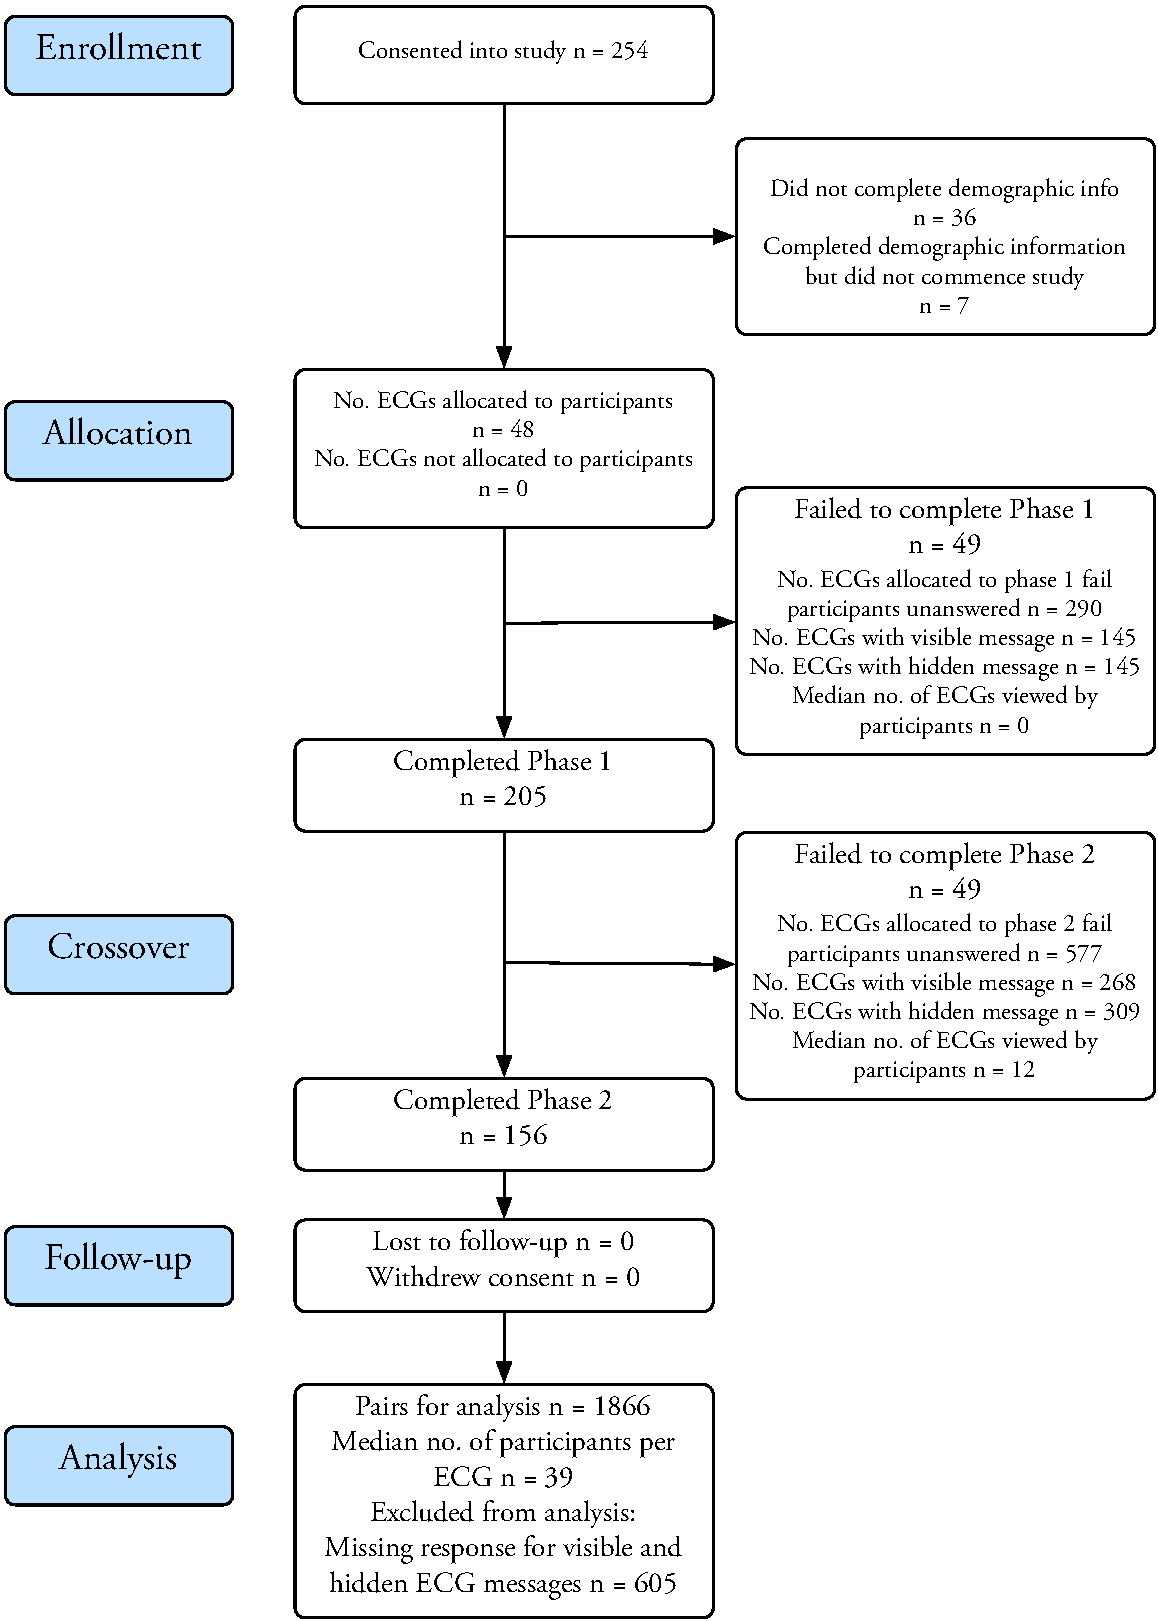
\includegraphics[keepaspectratio,width=\textwidth,height=0.9900\textheight,]{CONSORT-flow-diagram-pilot-completed.pdf}
\caption{CONSORT diagram for RESPECT pilot study}
\label{finalconsortpdf}
\end{figure}



 \newpage 

Demographic information was provided by 218 participants and this is summarised in \autoref{partcharfull}. There were 156 participants who completed both phases of the study and were included in the final analysis (\autoref{partcharfinish}), leaving 62 participants who did not complete the study (\autoref{partcharnofinish}). Aside from a lower median and interquartile range of CPD hours, they appear to have similar demographic characteristics. 

 % latex table generated in R 2.15.2 by xtable 1.7-1 package
% Mon Sep  2 18:40:13 2013
\begin{table}[htbp]
\centering
\caption{Summary of participant characteristics} 
\label{partcharfull}
\newcolumntype{K}{>{\centering\arraybackslash}p{0.13\textwidth}}
\newcolumntype{N}{>{\centering\arraybackslash}p{0.095\textwidth}}
\newcolumntype{B}{>{\arraybackslash}p{0.17\textwidth}}
\begin{tabular}{BKNNNNN}
  \hline
Characteristic & n & Lowest value & Lower quartile & Median & Upper quartile & Highest value \\ 
  \hline
Training route: &   &   &   &   &   &   \\ 
  Traditional & 134 (61\%) & - & - & - & - & - \\ 
  University & 84 (39\%) & - & - & - & - & - \\ 
  Service (yrs) & - & 0 & 2 & 5 & 10 & 32 \\ 
  CPD (hrs) & - & 0 & 1 & 4 & 10 & 160 \\ 
  pPCI patients & - & 0 & 2 & 4 & 6 & 41 \\ 
   \hline
\end{tabular}
\end{table}
 

 % latex table generated in R 2.15.2 by xtable 1.7-1 package
% Mon Sep  2 18:40:14 2013
\begin{table}[htbp]
\centering
\caption{Summary of participant characteristics who completed study} 
\label{partcharfinish}
\newcolumntype{K}{>{\centering\arraybackslash}p{0.13\textwidth}}
\newcolumntype{N}{>{\centering\arraybackslash}p{0.095\textwidth}}
\newcolumntype{B}{>{\arraybackslash}p{0.17\textwidth}}
\begin{tabular}{BKNNNNN}
  \hline
Characteristic & n & Lowest value & Lower quartile & Median & Upper quartile & Highest value \\ 
  \hline
Training route: &   &   &   &   &   &   \\ 
  Traditional & 96 (62\%) & - & - & - & - & - \\ 
  University & 60 (38\%) & - & - & - & - & - \\ 
  Service (yrs) & - & 0 & 2 & 5 & 10 & 32 \\ 
  CPD (hrs) & - & 0 & 2 & 5 & 11 & 160 \\ 
  pPCI patients & - & 0 & 1 & 3.5 & 5 & 41 \\ 
   \hline
\end{tabular}
\end{table}
 

 % latex table generated in R 2.15.2 by xtable 1.7-1 package
% Mon Sep  2 18:40:14 2013
\begin{table}[htbp]
\centering
\caption{Summary of participant characteristics who failed to complete study} 
\label{partcharnofinish}
\newcolumntype{K}{>{\centering\arraybackslash}p{0.13\textwidth}}
\newcolumntype{N}{>{\centering\arraybackslash}p{0.095\textwidth}}
\newcolumntype{B}{>{\arraybackslash}p{0.17\textwidth}}
\begin{tabular}{BKNNNNN}
  \hline
Characteristic & n & Lowest value & Lower quartile & Median & Upper quartile & Highest value \\ 
  \hline
Training route: &   &   &   &   &   &   \\ 
  Traditional & 38 (61\%) & - & - & - & - & - \\ 
  University & 24 (39\%) & - & - & - & - & - \\ 
  Service (yrs) & - & 0 & 2 & 5 & 10 & 30 \\ 
  CPD (hrs) & - & 0 & 0 & 2 & 6 & 120 \\ 
  pPCI patients & - & 0 & 3 & 4 & 6 & 30 \\ 
   \hline
\end{tabular}
\end{table}
 

\subsection{Incentives}
\label{incentives}

One of the aims of the pilot study was to examine the effect of incentives on attrition. To achieve this, participants were randomised into receiving one of the following incentive options:

\begin{itemize}
\item A CPD certificate

\item A prize draw for a paramedic textbook

\item Nothing.

\end{itemize}

\autoref{tableincentivefinal} shows the relation between randomised incentives and completion of the pilot study by participants. The chi-squared test for equality of proportions resulted in a p-value of 0.848, leading to the conclusion that there is no evidence that completion rates were dependent upon the incentive option.

\begin{table}[htbp]
\begin{minipage}{\linewidth}
\setlength{\tymax}{0.5\linewidth}
\centering
\small
\caption{Completion results by incentive offered}
\label{tableincentivefinal}
\begin{tabulary}{\textwidth}{@{}LLLL@{}} \toprule
&\multicolumn{2}{c}{Completed study}&\\
\textbf{Incentive}&\textbf{Yes}&\textbf{No}&\textbf{Total}\\
\midrule
Certificate&54 (74\%)&19 (26\%)&73\\
Prize draw&51 (71\%)&21(29\%)&72\\
None&51 (70\%)&22 (30\%)&73\\

\midrule
\textbf{Total}&156 (72\%)&62 (28\%)&218\\

\bottomrule

\end{tabulary}
\end{minipage}
\end{table}


\section{Electrocardiograms}
\label{electrocardiograms}

A complete set of summary statistics for each individual ECG, showing participant interpretation attempt and response times, can be found in \autoref{appendixh}. A concise synopsis of this data is shown in \autoref{meanpropecginteract}. 

 % latex table generated in R 2.15.2 by xtable 1.7-1 package
% Sat Aug 24 10:23:45 2013
\begin{table}[htbp]
\centering
\caption{Summary of participant interaction with ECGs} 
\label{meanpropecginteract}
\newcolumntype{D}{>{\arraybackslash}p{0.35\textwidth}}
                        \newcolumntype{E}{>{\centering\arraybackslash}p{0.1\textwidth}}
                        \newcolumntype{F}{>{\centering\arraybackslash}p{0.2\textwidth}}
                        \begin{tabular}{DEE|EE}
                       & \multicolumn{2}{F}{All data} & \multicolumn{2}{F}{Final data} \\
  \toprule
  & Median & Quartiles & Median & Quartiles \\ 
  \midrule
ECG interpretation attempts: total & 90 & 87-93 & 76 & 74-81 \\ 
  ECG interpretation attempts: message visible & 45 & 44-46 & 38 & 37-40 \\ 
  ECG interpretation attempts: message hidden & 44 & 42-46 & 38 & 37-41 \\ 
  Paired ECG interpretation attempts & 45 & 44-47 & 39 & 37-41 \\ 
   \bottomrule
\end{tabular}
\end{table}
 

The `All data' columns show the median and quartile values for an average ECG in the pilot study, when all ECG interpretation attempts are included. Final data, shows the same values, but only for the ECG interpretation attempts that were included in the final study analysis (i.e. after participants who had not completed both phases of the study were removed). There appears to be no evidence of differential completion rates between the message visibility of ECG interpretation attempts. A median of 39 paired ECG interpretation attempts for each ECG were available for the final analysis.

The boxplot figures (\autoref{boxplot1}, \autoref{boxplot2}, \autoref{boxplot3} and \autoref{boxplot4}) show the median ECG interpretation times by participant accuracy and computer interpretation for each ECG, sub-classified by message visibility. They demonstrate a wide range of ECG interpretation attempt completion times, suggesting that the time limit of 60 seconds, was appropriate.

 \begin{figure}[htbp]
\centerline{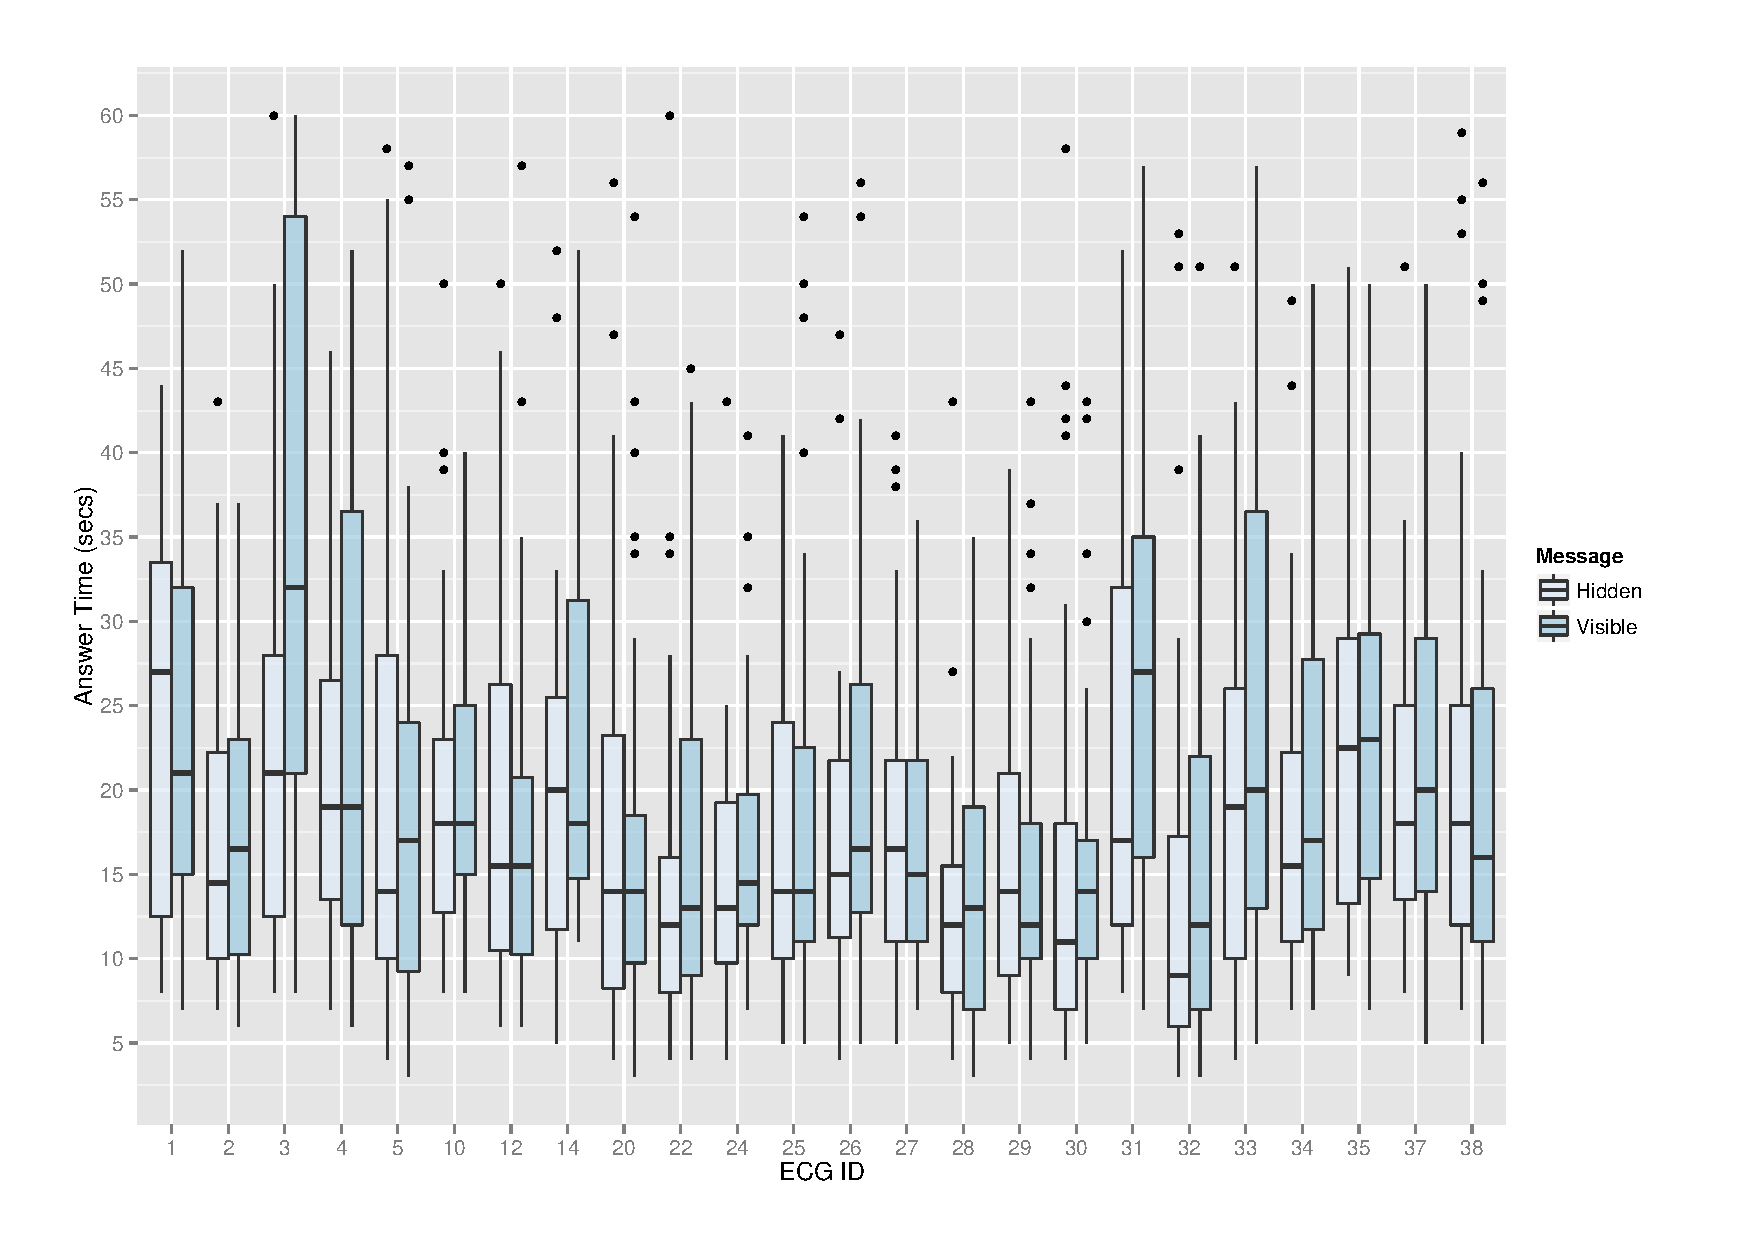
\includegraphics[page=1,keepaspectratio=false,width=0.8\paperwidth,height=0.45\paperwidth]{AnsTimeVsECG.pdf}}
\caption{Median answer time by ECG -- correct participant and computer interpretation}
\label{boxplot1}
\end{figure}

\begin{figure}[htbp]
\centerline{\includegraphics[page=2,keepaspectratio=false,width=0.8\paperwidth,height=0.45\paperwidth]{AnsTimeVsECG.pdf}}
\caption{Median answer time by ECG -- incorrect participant, and correct computer, interpretation}
\label{boxplot2}
\end{figure}

\begin{figure}[htbp]
\centerline{\includegraphics[page=3,keepaspectratio=false,width=0.8\paperwidth,height=0.45\paperwidth]{AnsTimeVsECG.pdf}}
\caption{Median answer time by ECG -- correct participant, and incorrect computer, interpretation}
\label{boxplot3}
\end{figure}

\begin{figure}[htbp]
\centerline{\includegraphics[page=4,keepaspectratio=false,width=0.8\paperwidth,height=0.45\paperwidth]{AnsTimeVsECG.pdf}}
\caption{Median answer time by ECG -- incorrect participant and computer interpretation}
\label{boxplot4}
\end{figure} 

 \newpage  

\section{Accuracy}
\label{accuracy}

\autoref{final2by2all} shows the sum totals of all responses by message visibility and answer accuracy. Participants in the pilot were correct approximately 80\% of the time, irrespective of whether the computer interpretation message was visible. 

\begin{table}[htbp]
\begin{minipage}{\linewidth}
\setlength{\tymax}{0.5\linewidth}
\centering
\small
\caption{Two-by-two table for all computer interpretations}
\label{final2by2all}
\begin{tabulary}{\textwidth}{@{}LCCC@{}} \toprule
&\multicolumn{2}{c}{Participant interpretation}&\\
Message&Correct&Incorrect&Total\\
\midrule
Visible&1481 (79\%)&385 (21\%)&1866\\
Hidden&1500 (80\%)&366 (20\%)&1866\\

\midrule
Total&2981(80\%)&751(20\%)&3732\\

\bottomrule

\end{tabulary}
\end{minipage}
\end{table}


When the data are split into correct and incorrect computer interpretations, a different pattern emerges. \autoref{final2by2correct} shows the results for ECGs with a correct computer interpretation. The results suggest that participants viewing this subset of ECGs, are more likely to make a correct interpretation. In addition, they are even more accurate when the computer interpretation message is visible.

\begin{table}[htbp]
\begin{minipage}{\linewidth}
\setlength{\tymax}{0.5\linewidth}
\centering
\small
\caption{Two-by-two table for all correct computer interpretations}
\label{final2by2correct}
\begin{tabulary}{\textwidth}{@{}LCCC@{}} \toprule
&\multicolumn{2}{c}{Participant interpretation}&\\
Message&Correct&Incorrect&Total\\
\midrule
Visible&816 (87\%)&117 (13\%)&933\\
Hidden&785 (84\%)&148 (16\%)&933\\

\midrule
Total&1601(86\%)&265 (14\%)&1866\\

\bottomrule

\end{tabulary}
\end{minipage}
\end{table}


Finally, \autoref{final2by2incorrect} shows the results for all ECGs with an incorrect computer interpretation. The results suggest that participants are less accurate in this sub-group, with 77\% of answers correct when the computer message is hidden, reducing to 71\% when the message is visible. 

\begin{table}[htbp]
\begin{minipage}{\linewidth}
\setlength{\tymax}{0.5\linewidth}
\centering
\small
\caption{Two-by-two table for all incorrect computer interpretations}
\label{final2by2incorrect}
\begin{tabulary}{\textwidth}{@{}LCCC@{}} \toprule
&\multicolumn{2}{c}{Participant interpretation}&\\
Message&Correct&Incorrect&Total\\
\midrule
Visible&665 (71\%)&268 (29\%)&933\\
Hidden&715 (77\%)&218 (23\%)&933\\

\midrule
Total&1380 (74\%)&486 (26\%)&1866\\

\bottomrule

\end{tabulary}
\end{minipage}
\end{table}


\section{Sensitivity and specificity}
\label{sensitivityandspecificity}

\autoref{partsensspec} shows the sensitivities and specificities for the participant responses, depending on computer interpretation accuracy and message visibility. There is little difference in sensitivity and specificity values, when participant ECG interpretation attempts of ECGs with correct and incorrect computer interpretation messages are analysed together.

  % latex table generated in R 2.15.2 by xtable 1.7-1 package
% Sun Aug 25 15:41:44 2013
\begin{table}[htbp]
\centering
\caption{Summary of sensitivities and specificities of participant responses} 
\label{partsensspec}
\newcolumntype{D}{>{\arraybackslash}p{0.3\textwidth}}
                        \newcolumntype{E}{>{\centering\arraybackslash}p{0.12\textwidth}}
                        \newcolumntype{F}{>{\centering\arraybackslash}p{0.24\textwidth}}
                        \begin{tabular}{DEE|EE}
                       & \multicolumn{2}{F}{Message Visible} & \multicolumn{2}{F}{Message Hidden} \\
  \toprule
Computer interpretation & Sensitivity & Specificity & Sensitivity & Specificity \\ 
  \midrule
All & 86 & 75 & 86 & 76 \\ 
  Correct & 92 & 85 & 89 & 80 \\ 
  Incorrect & 80 & 64 & 83 & 72 \\ 
   \bottomrule
\end{tabular}
\end{table}
  

However, if only the subgroup of participant interpretation attempts when the computer message is correct is considered, participants demonstrate a higher sensitivity and specificity, which increases further when the correct computer message is visible. Conversely, participant interpretation sensitivity and specificity decrease when only the ECGs which the computer interpreted incorrectly are included.

Overall, paramedics generally balance sensitivity and specificity quite well, with values around the 80\% mark, which is useful from a diagnostic perspective, but suggests that there is room for improvement. 

\section{Intra-class correlation coefficient}
\label{intra-classcorrelationcoefficient}

The intra-class correlation coefficient (ICC) is a measure of the degree of similarity between ECG interpretation attempts within a cluster. The ICC for participants is 0.05 and for ECGs, 0.41. The correlation between two randomly selected responses from the same participant, and the same ECG (known as the interaction ICC), was 0.46. These values suggest that taking clustering into account should make a significant difference in the GLM analysis.

\section{Generalised linear modelling results}
\label{generalisedlinearmodellingresults}

\autoref{ormesgall}, \autoref{ormesgcc} and \autoref{ormesgci} shows the results from the GLMs. The unadjusted odds ratios (OR) from the GLM are identical to those calculated from the two-by-two tables (\autoref{final2by2all}, \autoref{final2by2correct} and \autoref{final2by2incorrect}). Note that $ \sigma^2_{ecg}$ is the between-ECG variance for the random effects model and $ \sigma^2_{participant}$, the variance between participants. 

  % latex table generated in R 2.15.2 by xtable 1.7-1 package
% Sat Aug 24 13:35:11 2013
\begin{table}[htbp]
\centering
\caption{Odds ratio of correct interpretation} 
\label{ormesgall}
\begin{tabular}{lcccc}
  \toprule
Parameters & OR & z & P$>$$|z|$ & 95\% CI \\ 
  \midrule
\textit{Unadjusted for clustering}  &  &  &  & \\ 
  Constant & 4.10 & 24.20 & 0.00 & 3.66 to 4.60 \\ 
  Message & 0.94 & -0.78 & 0.44 & 0.80 to 1.10 \\ 
  \midrule
  \textit{Adjusted for clustering} &  &  &  & \\ 
  Constant & 6.48 & 9.42 & 0.00 & 4.39 to 9.56 \\ 
  Message & 0.92 & -0.88 & 0.38 & 0.77 to 1.10 \\ 
  \midrule 
  $\sigma^2_{ecg}$ & 1.57 &  &  &  \\ 
  $\sigma^2_{participant}$ & 0.21 &  &  &  \\ 
   \bottomrule
\end{tabular}
\end{table}
  

\autoref{ormesgcc} shows the odds ratio of a correct answer when the computer messages are correct. After adjusting for clustering, the odds ratio for the computer message has increased from 1.31 to 1.42. Conversely, in \autoref{ormesgci} it can be seen that the opposite result is obtained when the computer message is incorrect, as the odds ratio for the message decreases from 0.76 in the unadjusted model to 0.70 when clustering is taken into account.
  % latex table generated in R 2.15.2 by xtable 1.7-1 package
% Sat Aug 24 13:35:11 2013
\begin{table}[htbp]
\centering
\caption{Odds ratio of correct interpretation with correct computer message} 
\label{ormesgcc}
\begin{tabular}{lcccc}
  \toprule
Parameters & OR & z & P$>$$|z|$ & 95\% CI \\ 
  \midrule
\textit{Unadjusted for clustering}  &  &  &  & \\ 
  Constant & 5.30 & 18.62 & 0.00 & 4.46 to 6.35 \\ 
  Message & 1.31 & 2.05 & 0.04 & 1.01 to 1.71 \\ 
  \midrule
  \textit{Adjusted for clustering} &  &  &  & \\ 
  Constant & 9.16 & 8.32 & 0.00 & 5.43 to 15.43 \\ 
  Message & 1.42 & 2.36 & 0.02 & 1.06 to 1.89 \\ 
  \midrule 
  $\sigma^2_{ecg}$ & 1.57 &  &  &  \\ 
  $\sigma^2_{participant}$ & 0.21 &  &  &  \\ 
   \bottomrule
\end{tabular}
\end{table}
  

  % latex table generated in R 2.15.2 by xtable 1.7-1 package
% Sat Aug 24 13:35:12 2013
\begin{table}[htbp]
\centering
\caption{Odds ratio of correct interpretation with incorrect computer message} 
\label{ormesgci}
\begin{tabular}{lcccc}
  \toprule
Parameters & OR & z & P$>$$|z|$ & 95\% CI \\ 
  \midrule
\textit{Unadjusted for clustering}  &  &  &  & \\ 
  Constant & 3.28 & 15.35 & 0.00 & 2.82 to 3.82 \\ 
  Message & 0.76 & -2.63 & 0.01 & 0.61 to 0.93 \\ 
  \midrule
  \textit{Adjusted for clustering} &  &  &  & \\ 
  Constant & 4.95 & 5.80 & 0.00 & 2.88 to 8.49 \\ 
  Message & 0.70 & -3.03 & 0.00 & 0.56 to 0.88 \\ 
  \midrule 
  $\sigma^2_{ecg}$ & 1.57 &  &  &  \\ 
  $\sigma^2_{participant}$ & 0.21 &  &  &  \\ 
   \bottomrule
\end{tabular}
\end{table}
  

From the previous section, the ICC values suggested that the odds ratios would be significantly affected when clustering was taken into account. However, the odds ratios and confidence intervals from the GLM results do not appear to show this.
